\documentclass[11pt]{article}

%% Minimal packages
\usepackage[utf8]{inputenc}
\usepackage[T1]{fontenc}
\usepackage{lmodern}
\usepackage{amsmath,amssymb}
\usepackage{graphicx}
\usepackage{booktabs}

%% Custom commands
\newcommand{\proglang}[1]{\textsf{#1}}
\newcommand{\pkg}[1]{\textbf{#1}}
\newcommand{\code}[1]{\texttt{#1}}
\newcommand{\fct}[1]{\code{#1()}}
\newcommand{\class}[1]{`\code{#1}'}

%% Title
\title{\pkg{RcppML}: High-Performance Non-Negative Matrix Factorization\\
with Cross-Validation for \proglang{R}}

\author{Zachary DeBruine\\
University of Michigan\\
\texttt{debruine@umich.edu}}

\date{}

\begin{document}

\maketitle

\begin{abstract}
Non-negative matrix factorization (NMF) is a fundamental dimensionality 
reduction technique with applications spanning bioinformatics, text mining, 
computer vision, and signal processing. This paper presents \pkg{RcppML}, an 
\proglang{R} package that implements a comprehensive NMF framework with several 
key innovations: (1) a highly optimized sequential coordinate descent solver for 
non-negative least squares with support for L1 regularization and bounded 
solutions; (2) streaming cross-validation with minimal computational overhead 
using a novel position-dependent random number generator; (3) multiple robust 
loss functions including MSE, MAE, Huber, and KL-divergence implemented via 
iteratively reweighted least squares; (4) automatic rank determination through 
golden section search optimization; (5) specialized rank-2 NMF for 
high-performance spectral bipartitioning. The package provides unified support 
for both sparse and dense matrices through template metaprogramming and achieves 
state-of-the-art performance through careful cache-aware algorithm design.

\vspace{1em}
\noindent\textbf{Keywords:} non-negative matrix factorization, cross-validation, coordinate 
descent, spectral clustering, \proglang{R}, \proglang{C++}, \pkg{Rcpp}
\end{abstract}


%% =============================================================================
\section{Introduction}

Non-negative matrix factorization (NMF) decomposes a non-negative matrix 
$\mathbf{A} \in \mathbb{R}_{\geq 0}^{m \times n}$ into two non-negative factor 
matrices $\mathbf{W} \in \mathbb{R}_{\geq 0}^{m \times k}$ and 
$\mathbf{H} \in \mathbb{R}_{\geq 0}^{k \times n}$ such that 
$\mathbf{A} \approx \mathbf{W}\mathbf{H}$ (Lee and Seung, 1999). The non-negativity 
constraints enable parts-based, interpretable representations that have proven 
valuable across diverse domains including facial recognition, text mining, gene 
expression analysis (Brunet et al., 2004), and single-cell genomics.

The \pkg{RcppML} package for \proglang{R} addresses several practical challenges:

\begin{enumerate}
  \item \textbf{Integrated cross-validation}: A streaming algorithm that 
  computes held-out reconstruction error with minimal overhead ($<$5\% typical).
  
  \item \textbf{Robust loss functions}: Support for MSE, MAE, Huber, and 
  KL-divergence losses implemented via iteratively reweighted least squares 
  (IRLS).
  
  \item \textbf{Automatic rank determination}: Golden section search 
  optimization over the cross-validation objective to automatically identify 
  optimal rank.
  
  \item \textbf{Specialized rank-2 NMF}: A highly optimized implementation for 
  spectral bipartitioning that outperforms truncated SVD approaches.
  
  \item \textbf{High-performance implementation}: Cache-aware sequential 
  coordinate descent with unified support for sparse and dense matrices.
\end{enumerate}


%% =============================================================================
\section{NMF Algorithm}

\subsection{Problem Formulation}

We formulate NMF with a scaling diagonal:
\begin{equation}
  \min_{\mathbf{W}, \mathbf{D}, \mathbf{H}} 
  \mathcal{L}(\mathbf{A}, \mathbf{W}\mathbf{D}\mathbf{H}) + 
  \lambda_1 \|\mathbf{W}\|_1 + \lambda_1 \|\mathbf{H}\|_1
\end{equation}
subject to $\mathbf{W}, \mathbf{H} \geq 0$, $\mathbf{D} = \text{diag}(d_1, 
\ldots, d_k)$, and optional column normalization $\|\mathbf{w}_j\|_2 = 1$.

\subsection{Alternating Least Squares}

We optimize using alternating least squares (ALS), iteratively solving:
\begin{align}
  \mathbf{H} &\leftarrow \arg\min_{\mathbf{H} \geq 0} 
  \|\mathbf{A} - \mathbf{W}\mathbf{D}\mathbf{H}\|_F^2 + \lambda_1\|\mathbf{H}\|_1 \\
  \mathbf{W} &\leftarrow \arg\min_{\mathbf{W} \geq 0} 
  \|\mathbf{A}^\top - \mathbf{H}^\top\mathbf{D}\mathbf{W}^\top\|_F^2 + 
  \lambda_1\|\mathbf{W}\|_1
\end{align}

\subsection{Sequential Coordinate Descent Solver}

We solve NNLS using sequential coordinate descent (Franc et al., 2005):
\begin{equation}
  h_i \leftarrow \max\left(0, \frac{\mathbf{w}_i^\top(\mathbf{a} - 
  \tilde{\mathbf{W}}\mathbf{h}) + h_i \|\mathbf{w}_i\|_2^2 - \lambda_1}
  {\|\mathbf{w}_i\|_2^2}\right)
\end{equation}

The key insight is to maintain the residual $\mathbf{r} = \mathbf{a} - 
\tilde{\mathbf{W}}\mathbf{h}$ incrementally, reducing the complexity of each 
coordinate update from $O(mk)$ to $O(m)$.


%% =============================================================================
\section{Cross-Validation Framework}

\subsection{Position-Dependent Random Masking}

We use a position-dependent random number generator that deterministically 
determines whether each entry is masked based on its position $(i, j)$:
\begin{equation}
  \text{mask}(i, j) = \mathbf{1}[\text{hash}(i, j, \text{seed}) < p_{\text{cv}}]
\end{equation}

This ``speckled'' RNG has several advantages: (1) no memory allocation for the 
mask; (2) the same entry maps to the same mask value throughout optimization; 
(3) reproducibility through the seed.

\subsection{Streaming Loss Accumulation}

During each ALS iteration, we accumulate test error ``for free'' within the 
NNLS solve by checking the mask and accumulating squared residuals. This 
streaming approach has $O(1)$ memory overhead.


%% =============================================================================
\section{Loss Functions}

\pkg{RcppML} supports four loss functions via IRLS:

\begin{itemize}
  \item \textbf{MSE}: $\rho(r) = r^2$, $w(r) = 1$
  \item \textbf{MAE}: $\rho(r) = |r|$, $w(r) = 1/(|r| + \varepsilon)$
  \item \textbf{Huber}: Interpolates between L2 and L1
  \item \textbf{KL-divergence}: For count data
\end{itemize}


%% =============================================================================
\section{Automatic Rank Determination}

When the rank is unknown, \pkg{RcppML} supports automatic selection via 
\code{k = "auto"}. This performs golden section search over the 
cross-validation objective:
\begin{equation}
  k^* = \arg\min_{k \in [k_{\min}, k_{\max}]} \text{CV-MSE}(k)
\end{equation}


%% =============================================================================
\section{Rank-2 NMF for Spectral Bipartitioning}

The \fct{bipartition} function implements a highly optimized rank-2 NMF 
for spectral bipartitioning. Given $\mathbf{A} \in \mathbb{R}_{\geq 0}^{m \times n}$, 
it returns a vector $\mathbf{v} \in \{-1, +1\}^n$ indicating cluster membership.

Table~\ref{tab:bipartition} compares \fct{bipartition} to \fct{irlba}.

\begin{table}[t]
\centering
\begin{tabular}{lrrr}
\toprule
Matrix size & Density & \fct{bipartition} (ms) & \fct{irlba} (ms) \\
\midrule
$1000 \times 500$ & 10\% & 17 & 25 \\
\bottomrule
\end{tabular}
\caption{Runtime comparison for rank-2 factorization.}
\label{tab:bipartition}
\end{table}

The \fct{dclust} function builds on \fct{bipartition} to perform divisive 
hierarchical clustering using modularity as the stopping criterion.


%% =============================================================================
\section{Illustrations}

\subsection{Cross-Validation for Rank Selection}

Figure~\ref{fig:cv} shows typical cross-validation curves. The test MSE 
decreases as rank increases then increases (overfitting).

\begin{figure}[t]
\centering
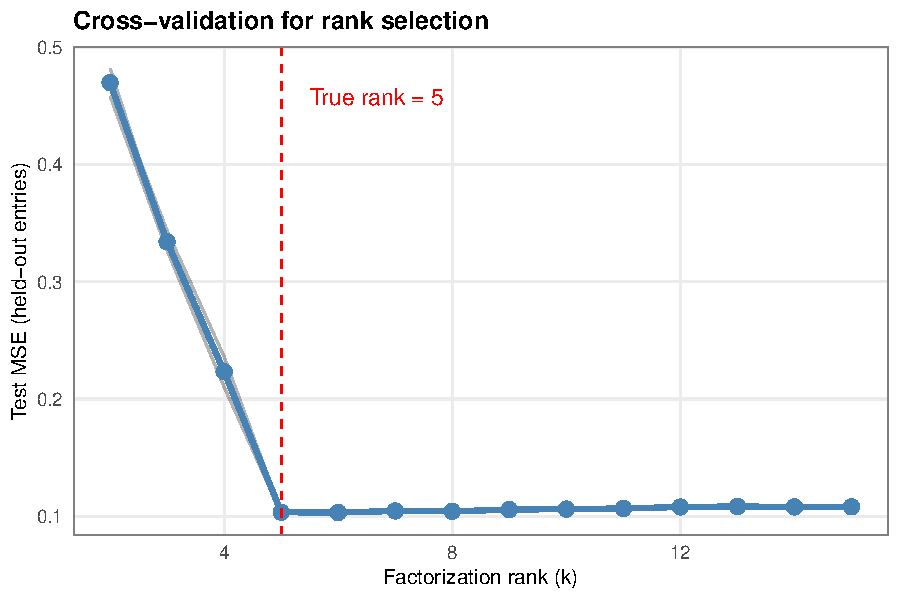
\includegraphics[width=0.8\textwidth]{fig_cv_rank}
\caption{Cross-validation for rank selection on synthetic data 
with true rank 5. Test MSE is minimized near the true rank.}
\label{fig:cv}
\end{figure}

\subsection{Regularization Effects}

Figure~\ref{fig:l1} shows the trade-off between reconstruction error and 
factor sparsity under L1 regularization.

\begin{figure}[t]
\centering
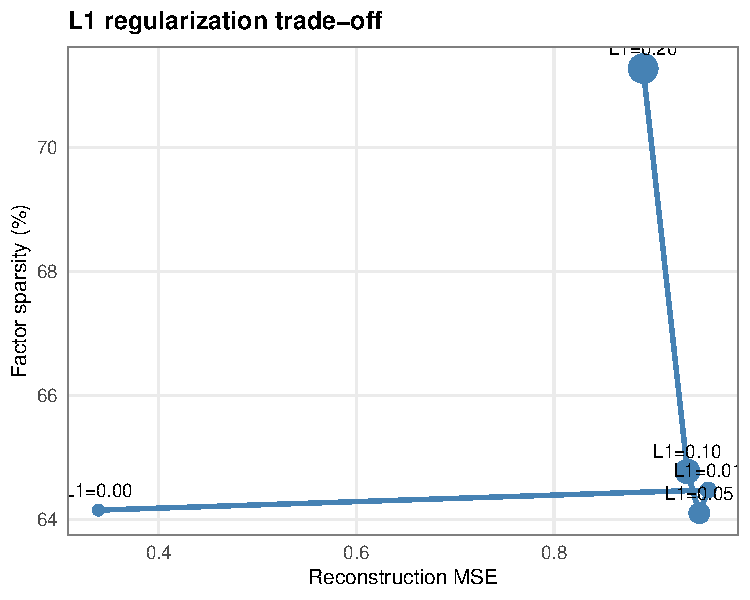
\includegraphics[width=0.7\textwidth]{fig_l1_tradeoff}
\caption{L1 regularization trade-off.}
\label{fig:l1}
\end{figure}

\subsection{Scaling Behavior}

Figure~\ref{fig:scaling} shows runtime scaling for sparse and dense matrices.

\begin{figure}[t]
\centering
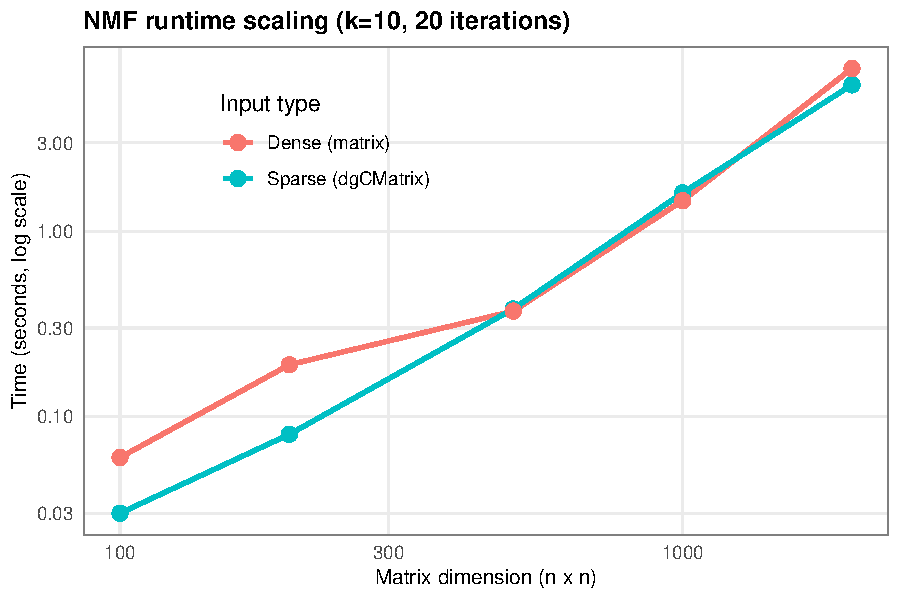
\includegraphics[width=0.8\textwidth]{fig_scaling}
\caption{Runtime scaling for NMF on sparse and dense matrices.}
\label{fig:scaling}
\end{figure}


%% =============================================================================
\section{Summary}

The \pkg{RcppML} package provides a comprehensive NMF implementation for 
\proglang{R} with integrated cross-validation, multiple loss functions via IRLS, 
automatic rank determination through golden section search, and specialized 
rank-2 NMF for spectral bipartitioning. The package is available on CRAN.


%% -- Computational details ----------------------------------------------------

\section*{Computational Details}

The results in this paper were obtained using \proglang{R}~4.5.0 with the 
packages \pkg{RcppML}~1.0.0, \pkg{Matrix}~1.7.3, \pkg{irlba}~2.3.5.1, and 
\pkg{ggplot2}~4.0.1.

\section*{References}

\begin{itemize}
\item Brunet, J.-P., Tamayo, P., Golub, T. R., and Mesirov, J. P. (2004). 
Metagenes and molecular pattern discovery using matrix factorization. 
\emph{PNAS}, 101(12):4164--4169.

\item Eddelbuettel, D. and Fran\c{c}ois, R. (2011). 
Rcpp: Seamless R and C++ integration. 
\emph{Journal of Statistical Software}, 40(8):1--18.

\item Franc, V., Hlavac, V., and Navara, M. (2005). 
Sequential coordinate-wise algorithm for the non-negative least squares problem.
\emph{CAIP 2005}, pages 407--414.

\item Lee, D. D. and Seung, H. S. (1999). 
Learning the parts of objects by non-negative matrix factorization. 
\emph{Nature}, 401(6755):788--791.
\end{itemize}

\end{document}
